% 
% Annual Cognitive Science Conference
% Sample LaTeX Paper -- Proceedings Format
% 

% Original : Ashwin Ram (ashwin@cc.gatech.edu)       04/01/1994
% Modified : Johanna Moore (jmoore@cs.pitt.edu)      03/17/1995
% Modified : David Noelle (noelle@ucsd.edu)          03/15/1996
% Modified : Pat Langley (langley@cs.stanford.edu)   01/26/1997
% Latex2e corrections by Ramin Charles Nakisa        01/28/1997 
% Modified : Tina Eliassi-Rad (eliassi@cs.wisc.edu)  01/31/1998
% Modified : Trisha Yannuzzi (trisha@ircs.upenn.edu) 12/28/1999 (in process)
% Modified : Mary Ellen Foster (M.E.Foster@ed.ac.uk) 12/11/2000
% Modified : Ken Forbus                              01/23/2004
% Modified : Eli M. Silk (esilk@pitt.edu)            05/24/2005
% Modified : Niels Taatgen (taatgen@cmu.edu)         10/24/2006
% Modified : David Noelle (dnoelle@ucmerced.edu)     11/19/2014

%% Change "letterpaper" in the following line to "a4paper" if you must.

\documentclass[10pt,letterpaper]{article}
\usepackage{graphicx}
\usepackage{cogsci}
\usepackage{pslatex}
\usepackage{apacite}
\usepackage{color}
\usepackage{url}
%\usepackage{hyperref}
%\hypersetup{
%    colorlinks=true,
%    linkcolor=blue,
%    filecolor=magenta,      
%    urlcolor=cyan,
%}

\definecolor{Red}{RGB}{255,0,0}
\newcommand{\red}[1]{\textcolor{Red}{#1}}  



\title{Understanding the Costs and Benefits of Learning When Teaching Others}
 
\author{{\large \bf Sophie Bridgers (sbridge@stanford.edu)} \\
  Department of Psychology, Jordan Hall, 450 Serra Mall \\
 Stanford, CA 94305 USA
  \AND {\large \bf Emily Tang (emjtang@stanford.edu)} \\
   Department of Psychology, Jordan Hall, 450 Serra Mall \\
 Stanford, CA 94305 USA}

\begin{document}

\maketitle


\begin{abstract}
To-Do

\textbf{Keywords:} 
pedagogy; social learning; cost-benefit analysis; Bayesian models
\end{abstract}


\section{Introduction}

Teaching is one of the most powerful forms of human communication, enabling a rapid, effective dissemination of knowledge and culture within and across generations. Remarkably, we decide what information to teach without direct access to the learner's mind and often without explicit requests for information. How do we make this inference and how does this capacity develop? 

Consider a naive learner who encounters a novel toy and tries to figure out how it works via self-guided exploration. The learner likely has her own ideas about how the toy works and will test these hypotheses by intervening on the toy. However, this generation of evidence is costly, requiring time and effort. Additionally, the value of this exploration is uncertain as the learner might never successfully activate the toy. Teachers can help decrease the costs of learning by communicating information that would be too difficult, time-consuming, or perhaps even impossible to obtain on one's own. Likewise, teachers can increase the value of learning by providing the critical information needed to support the most accurate inference. Thus, an effective teacher should be sensitive to opportunities for maximizing the benefits of learning (the value of the information gained) and minimizing its costs (the effort needed to acquire it). However, neither the costs nor benefits of learning are directly observable; one must consider the learner's prior knowledge and goals, and reason forward in time to calculate the expected costs and benefits of learning.

Prior research suggests that even young children might be capable of such a sophisticated inference. Both infants and children expect agents to act in accordance with the principle of rationality -- i.e., that agents will act efficiently in pursuit of their goals \cite{Baker2009}. 
Looking time studies reveal that infants anticipate an agent to choose the action requiring the least amount of effort to achieve her goal \cite{Scott2013}.
Preschool-aged children, like adults, go beyond simply reasoning about the overall utility of agents' goal-directed actions. 
Rather, they consider the relative costs and rewards of pursuing certain goals over others and make judgments consistent with a naive utility calculus, expecting agents to incur higher costs for greater rewards \cite{JaraEttinger2015}.

Relatedly, children and adults consider both the value and costs of information transfer when evaluating teachers, preferring teachers who provide enough evidence to support accurate inference over those who are exhaustively informative \cite{GweonReview, Shafto2012}. Likewise, children can decide how much information to teach given the learner's prior knowledge and goals and the costs of information transfer: If the learner has relevant prior knowledge, children are selective in how much they teach unless providing exhaustive information is no more costly (i.e., they are allowed to verbally explain how a toy works rather than needing to physically demonstrate it)  \cite{GweonSchulz2014}. Building upon this work, Bridgers and Gweon hypothesize that children (and adults) can flexibly decide what information to teach via an intuitive cost-benefit analysis. More specifically, they predict that children (5 to 7 years old) reason about the expected benefits and costs of learning on one's own (from the perspective of the learner), and successfully choose to teach information that maximizes the benefits and minimizes the costs. 

In a current experiment, Bridgers and Gweon are investigating whether children selectively teach information that decreases the expected costs of learning. In this study, children explore two novel toys. One toy has an obvious causal mechanism that is easy to discover and that produces an exciting effect (a single, red button that causes the toy to light-up and spin). The other toy has a non-obvious mechanism that is difficult to discover without instruction and that produces a relatively less interesting effect (two of seven buttons must be pressed simultaneously to make the toy play music). Once children learn how the toys work, they are asked to choose one to teach to a naive learner who will play with the toys later all by herself. Given children's sensitivity to differences in the costs of verbal communication and additional actions on a toy, Bridgers and Gweon predict children will reason about the expected costs of figuring out the toys on one's own vs. from instruction and will more often teach the difficult toy than the easy toy, but not in the control condition where each toy is equally easy to figure out.

Here, we formalize the intuitions Bridgers and Gweon investigate with a computational theory of efficient teaching. We develop a Bayesian cognitive model of a knowledgeable teacher reasoning about a naive learner who wants to figure out how two toys work. In this simplified scenario, the teacher selects one of two toys to teach the learner and the learner discovers how the other toy works on her own. We assume the teacher is helpful and that her goal is to teach the toy that will maximize the probability that the learner figures out how to activate both toys. The teacher, thus, critically bases her decision on the relative costs for the learner of figuring out how the toys work without instruction. 

In this paper, we first describe the details of the model and show that it predicts the teacher will teach the toy that has a higher cost of learning but when costs are equal, the toy with the higher value. \textcolor{red}{I thought that the model is at chance when the toys are matched in costs, and doesn't return the toy with the higher value?} Second, we compare the model's predictions to adult performance in an experiment based on Bridgers and Gweon's experiments with children. Finally, we conclude by discussing how the predictions of the model help us to better understand how we decide what to teach and how the model could be extended to incorporate the teacher's reasoning about her own costs and benefits of teaching to better account for the dyadic nature of pedagogical interactions.

\section{Model}

Central to our modeling approach are the ideas discussed in chapter 6 (Inference about inference) of Probabilistic Models of Cognition \cite{Goodman}. Our efficient teaching model merges the vending machine model and the teacher-learner model (both presented in chapter 6).  We modified the 'make-vending-machine' function to a 'make-toy' function: toys take a single action as an argument and return either an effect or nothing. Each possible action on a toy has a certain probability of producing the effect. Put simply, each toy has one to multiple buttons, and when pressed these buttons produce an outcome (e.g., something lights up) with high probability (90\%) or low probability (10\%). In the scenarios we consider, there are always two toys, which we will refer to as toy A and toy B, varying in learning cost and value (e.g., a toy that is easy to learn but high in value versus a toy that is hard to learn but low in value). The cost of learning is represented as the uncertainty over what action will cause the toy to produce an outcome; thus, cost increases as the number of buttons (possible actions) increases. The value of learning is represented as the quantity of the outcome (currently the number of lights). For all of the toys we consider, one button produces the effect(s) with high probability and all additional buttons with low probability.

The learner is represented as a function that takes in her goal (to activate both toys) and a message from the teacher about how one of the two toys works. Prior to receiving the teacher's message, the learner does not know how either of the toys works (expressed as not knowing the probability of effect associated with the possible actions on each toy).  As a result of the teacher's message, the learner knows how one toy works but does not know about the other toy and will need to figure it out on her own. We query the learner model for the actions she takes on toy A and toy B conditioning on her goal being satisfied (i.e., that she successfully activates the toys). The learner function thus returns the probability that the learner will successfully activate both toys, $a$, given the message the teacher sends about one toy, $t$, and the learner's goal of activating both, $g_{learner}$ ($P_{learner}(a | t, g_{learner})$). 

The teacher is represented as a function with no arguments. The teacher knows how both toy A and toy B works (expressed as having knowledge of the probability of effect for each possible action on the toys). The teacher also has knowledge of the learner's goal to activate both toys. The learner's goal is represented within the teacher-model as a boolean utility function that takes the outcomes of the learner's actions on each toy as arguments. The function returns true if the learner's actions bring about an effect \textcolor{red}{in both toys(?)} and false otherwise. We assume that the learner wants to maximize the reward of her actions and see the highest possible number of effects (e.g., the highest number of lights); however, we also assume that the learner is \textit{soft-max} optimal. We implement this notion in the model by making the conditions that satisfy the learner's goal probabilistic: the learner's goal function is most likely to return true if the learner's actions bring about the maximal effect across the two toys, but sometimes it returns true for sub-optimal returns. 

We assume the teacher is helpful and that her goal is for the learner to figure out how both toys work (i.e., that the learner will perform an action on each toy that successfully brings about an effect). The teacher's goal is also represented as a boolean function that takes the learner's actions on the toys as arguments and returns true (i.e, the goal is satisfied) if these actions bring about an effect and false otherwise. Similar to our assumptions about the learner, we assume the teacher is \textit{soft-max} optimal and implement this notion in the same way we do for the learner. 

However, though the teacher wants the learner to successfully activate both toys, the teacher can only teach the learner how \textit{one} of the toys works. We formalize this constraint as the teacher sends the button-effects for one toy and "naive-notions" of the button effects for the other toy (i.e., that each button on this toy is equally likely to bring about the effect). Thus, the teacher must decide to teach the toy that will maximize the probability that the learner will successfully activate both toys; we expect the teacher to select the toy that reduces the greatest amount of uncertainty for the learner about how the toys work. We query the teacher model for the toy she teaches (i.e., the message with the button-effects for \textit{either} toy A or toy B that she sends to the learner-model), and we condition on her goal being satisfied. The teacher function thus returns the probability that the teacher will teach one of the toys, $t$, given the teacher's goal, $g_{teacher}$, defined in terms of the effects the learner's actions (based on the teacher's message) achieve ($P_{teacher}(t | g_{teacher})$).

For complete details on how we implement our model of efficient teaching, please see \url{https://github.com/sbridgers/Psych204_Experiment_and_Model/blob/master/ModelCode/TeacherModel.md} for the model online.

\subsection{Model Predictions}

We test the predictions of our model for a series of scenarios comparing toys varying in expected learning cost and value. We find that for each of these scenarios, the model's predictions are consistent with our intuitions. 

We first see what the model predicts the teacher will teach when choosing between two toys equal in cost but unequal in value. We find, as we would expect, that the model does not make a strong prediction in this scenario: the probability that the teacher teaches each of the toys is approximately 50\%. Next, we see what the model predicts when toy A and toy B are equal in cost (e.g., they each have two buttons) but unequal in value (e.g., toy A produces two effects, while toy B only produces one). We find that in this scenario, the teacher teaches toy A with a higher probability than toy B ($P(toyA) \sim 57\%$). \textcolor{red}{<< wait this seems contradictory? is the first sentence referring to two toys equal in LOW cost and then the second scenario a higher equal cost (both toys have two buttons)? it's a little confusing}

When choosing between two toys unequal in cost but equal in value, the model predicts the teacher will teach the toy with the higher expected cost of learning. For example, if both toys produce two effects but toy A has one button, while toy B has 7, the model predicts the teacher will teach toy B with higher probability than toy A ($P(toyB) \sim 60\%$). Relatedly, if toy B is associated with the higher cost \textit{and} the higher value (e.g., toy B has 7 buttons and produces two effects, while toy A has one button and only produces one effect), the model again predicts the teacher will teach toy B with higher probability than toy A ($P(toyB) \sim 65\%$).

Thus far the scenarios we have considered have fairly straight forward intuitive predictions, and we have shown that the model's predictions match our own. When the toys are matched in cost and value, the model predicts that teacher will teach each toy with equal probability. When the toys are matched in value, but unequal in cost, the model predicts that the teacher will teach the toy with higher cost with greater probability than the toy with lower cost. When the toys are mis-matched in value and unequal in cost, the model predicts that the teacher will most probably teach the toy with higher cost when that toy also has the higher value. But what about when the toy with higher cost is lower in value than the toy with lower cost? What toy should the teacher teach: the toy that has a higher expected value of learning or the toy that has a higher expected cost? We assume that in this scenario teaching the toy with higher cost is the most helpful because it reduces the greatest amount of uncertainty for the learner and maximizes the probability that she will be able to successfully activate \textit{both} toys. We find that the model's predictions here are again consistent with our intuitions: when toy B is higher in cost but lower in value than toy A, the model predicts the teacher will teach toy B with a higher probability than toy A ($P(toyB) \sim 55\%$).

\section{Experiment 1: Testing Adult Intuitions}

In the current experiment, we aimed to validate the predictions of our model with adult performance. The experiment was based on Bridgers and Gweon's experiments with children. Adults were presented with pairs of toys varying in relative cost and value. We selected three scenarios considered in the modeling section above: (1) two toys equal in low cost but unequal in value, (2) two toys unequal in cost but equal in low value, (3) and one toy low in cost but high in value versus one toy high in cost but low in value. After exploring the toys and figuring out how they worked, adults were asked to choose one of the toys to teach to a child learner who did not know how either of the toys worked but wanted to activate both of them. 

\subsection{Method}

\subsubsection{Participants}

Ninety adults were tested via an online survey on Amazon Mechanical Turk. Participants were paid \$0.30 for their time. Participation was restricted to Amazon Mechanical Turk workers who had a HIT acceptance rate of $\sim 95\%$ and a U.S. IP address. Nine participants were excluded either due to failing the first catch-trial (described below) or explicitly commenting that they had experienced technical difficulties with the survey. The final sample included 81 participants ($\sim 46\%$ female). Participants were randomly assigned to one of three conditions: the Equal Low Cost and Unequal Value condition ($n = 36$), the Unequal Cost and Equal Low Value condition ($n = 24$), and the Unequal Cost and Unequal Value condition ($n = 21$). 

\subsubsection{Stimuli}

The stimuli were adapted from those used by Bridgers and Gweon in their current experiments with children. Each toy was represented as a rectangular blue box, with a certain number of light bulbs and a certain number of either red or yellow buttons on top. Only one button activated the light bulb(s) on each toy. A toy's value was represented by the number of light bulbs: the high value toys had two light bulbs and the low value toys had one light bulb. A toy's cost was represented by the number of buttons:. the high cost toys had ten buttons and the low cost toys had one button. Toy A always had red buttons and was always low in cost but varied in value. Toy B always had yellow buttons and was always low in value but varied in cost.

\subsubsection{Procedure}

Participants were first introduced to two toys, Toy A and Toy B, and were told that it was their job to figure out how these toys worked. Toy A was always presented on the left of the screen, and Toy B was always presented on the right. In the Equal Low Cost and Unequal Value condition, the two toys were matched in (low) cost (i.e., they both had one button), but differed in value (i.e., Toy A had two light bulbs, while Toy B had one). In the Unequal Cost and Equal Low Value condition, the two toys were matched in (low) value (i.e., both had one light-bulb), but differed in cost (i.e., Toy A had one button, low cost and Toy B had ten buttons, high cost). Finally, in the Unequal Cost and Unequal Value condition, the two toys differed in both value and cost: Toy A had one button but two light-bulbs (low cost, high value) and Toy B had ten buttons and one light-bulb (high cost, low value). 

Adults were then encouraged to virtually interact with and explore each toy. The toys were presented one at time (Toy A always came first); numbered buttons that corresponded to the actual buttons on top of the toy were displayed below the toy. Participants could use their mouse to click on these buttons and see what happened to the toy. If participants clicked the activator button, the light-bulb(s) would flash on for approximately one second. When Toy B was high in cost, button 4 was always the activator button. There was no time limit for this exploration, and participants were not permitted to advance until they successfully activated the toy. 

Once adults activated the toy correctly, they were asked a to enter the number of the activator button in a text box. Since Toy A only ever had one button, participants who failed to answer this catch-trial correctly were excluded from analysis. Overall, participants' memory for the activator button on Toy B was low, so for the purposes of this experiment, we did not exclude these participants. After successfully activating both toys and completing the catch-trials, adults were then introduced to Ollie, a naive, child learner whose goal was to activate both toys. Specifically, participants were told: ``Ollie does not know how these toys work. But he really wants to make \textbf{both} of the toys go. You can help Ollie and \textbf{teach} him how \textbf{ONE of these toys} works. He will try the other toy by \textbf{himself}." Adults were then instructed to select just one of the two toys to teach Ollie; adults made their selection by clicking on a radio button underneath the image of the toy they had chosen. 

After deciding what to teach, adults were asked to rate how confident they were in their choice on a horizontal slider bar from ``Not at all confident" to ``Really confident". Participants were also asked to explain why they chose to teach one toy over the other, and then were asked to categorize their free-response explanation by completing the statement, ``I chose to teach Ollie this toy because", with one of the following options: a) the toy has cooler effects, b) the toy is harder to figure out, c) the toy has cooler effects and is harder to figure out, d) not sure why, and e) none of the above apply. Lastly, adults answered two questions: (1) ``Which toy was harder to figure out?" and (2) ``Which toy has the cooler effect?" by rating on a horizontal slider bar from ``Definitely Toy A" to ``Definitely Toy B". For more details, the current experiment can be viewed online here:  \url{http://web.stanford.edu/~sbridge/experiments/teaching-toys/Psych204_Experiment_and_Model/Experiment/experiment/toyExperiment.html}.

\subsection{Results}

Adult performance is summarized in Figure 1. In the Unequal Cost and Equal Low Value condition, a higher proportion of adults chose to teach the high cost toy (Toy B) over the low cost toy (Toy A); however, this difference was not significant (two-tailed binomial test, \textcolor{red}{there was a space here! is there supposed to be something else?}). In the Equal Low Cost and Unequal Value condition, adults were significantly more likely to teach the low value toy (Toy B) over the high value toy (Toy A) (two-tailed binomial test, \textcolor{red}{also here}). Finally, in the Unequal Cost and Unequal Value condition, a higher proportion of adults chose to teach the low cost, high value toy (Toy A) over the high cost, low value toy (Toy B); however, this difference was not significant (two-tailed binomial test,\textcolor{red}{actually it seems like you're going to add the test results here...}). We also conducted a logistic regression with condition as a single predictor of participants' responses to the teach question. This model revealed that participants in the Equal Low Cost and Unequal Value condition were significantly more likely to select to teach Toy B, than participants in the Unequal Cost and Unequal Value condition ($b = , z() = , p = $). Participants in the Unequal Cost and Equal Low Value condition, on the other hand, did not select to teach Toy B significantly more often than participants in the Unequal Cost and Unequal Value condition ($b = , z() = , p = $). A t-test revealed that there was also no difference in participants' responses to the teach question between the Equal Low Cost and Unequal Value condition and the Unequal Cost and Equal Low Value condition ($t(46.8) = 0.861,  p-value = 0.39$). In other words...

\begin{figure}[ht]
\begin{center}
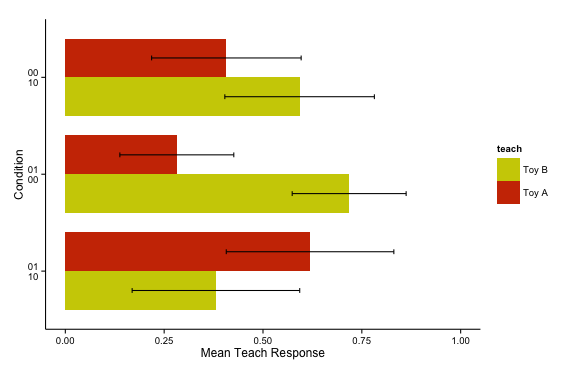
\includegraphics[width=10cm]{cleanHorizontalBarplot_n87.png}
\end{center}
\caption{The proportion of adults who chose to teach Toy A (in red) or Toy B (in yellow) in each condition. The top bars are from the Unequal Cost and Equal Low Value condition, the middle bars are from the Equal Low Cost and Unequal Value condition, and the bottom bars are from the Unequal Cost and Unequal Value conditions. Error bars are $95\%$ CI.} 
\label{Figure 1}
\end{figure}

\begin{figure}[ht]
\begin{center}
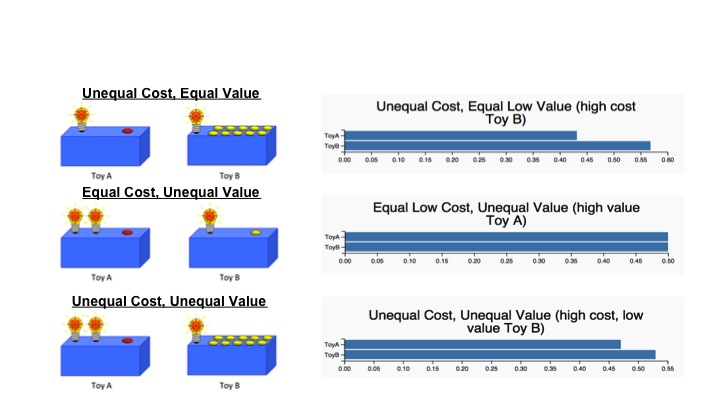
\includegraphics[width=9cm]{modelPredictions.png}
\end{center}
\caption{Summary of model predictions for the three conditions tested with adults. Schematics of the two toys used in each condition are displayed to the left of the model predictions for that condition.} 
\label{Figure 2}
\end{figure}

\subsubsection{Comparing Model Predictions with Adult Performance}
ADD IN NUMBERS
Our model predictions are consistent with adult performance for the Unequal Cost and Equal Low Value condition, both qualitatively and quantitatively. A higher proportion of adults in this condition chose to teach the high cost toy, Toy B, than chose to teach the low cost toy, Toy A. Our model predicted this as well: the high cost toy (which has a higher number of buttons than the low cost toy) is probabilistically more difficult to figure out and there is a higher degree of uncertainty whether the child learner will successfully activate this toy. Thus, our model predicted that the teacher would more often select to teach Toy B since teaching this toy reduces the greatest amount of uncertainty for the learner and maximizes the probability that the learner will figure out both toys. 

For the other two conditions, the adult performance deviates from our model predictions. In the Equal Low Cost and Unequal Value condition, adults were more likely to choose to teach the low value toy rather than the high value toy, while our model predicted that adults would select to teach either toy with equal probability. Our model makes this prediction because there is only one button on each toy, so there is no uncertainty that the learner will successfully activate both toys regardless of which toy is taught.

In the Unequal Cost and Unequal Value condition, more adults chose to teach the low cost, high value toy than the high cost, low value toy, whereas our model predicted performance in the opposite direction (i.e., that adults would teach the high cost, low value toy, Toy B, with higher probability than the low cost, high value toy, Toy A). Our model makes this prediction because although Toy A is higher in value, there is a greater uncertainty with Toy B that the learner will successfully activate the toy, so teaching this toy maximizes the probability that the learner will successfully fulfill his goal of activating both toys.

\subsection{General Discussion}

Adults in our experiment were indeed sensitive to the choice of toys presented, and their teaching decisions varied depending on how the two toys differed, though not always in the predicted direction. When adults were presented with two toys that were both low in value (each had one light bulb) but differed in learning costs (one toy had one button, while the other toy had 10), adults were sensitive to this difference in learning costs and a higher proportion chose to teach the high cost (harder) toy to Ollie, our naive learner. We should note that this difference in adult performance was not significant, likely due to our small sample size and high variance in response type. Adult performance in this condition was also consistent with our model predictions. Anecdotally, adults' explanations for why they chose to teach the high cost toy, appeal to the difficulty of the toy and how much time it would take Ollie to figure it out. Examples of such explanations include: ``it's more complex" or as one subject eloquently put it: ``I chose to teach Ollie this toy because it has 10 buttons and it is much better for me to teach him which one makes the toy "go" so he doesn't have to spend time on it; Toy A only has one button so he will press it and it will light up. There's nothing really to teach him about Toy A." In sum, the results of this condition indicate that adults do consider how difficult or costly things are to learn from the perspective of the learner and select to teach information that minimizes these costs. 

Our model predicted that when given an opportunity to teach one of two toys that were equal in cost (each had one button and so were low in learning cost) but different in value (one toy had two light-bulbs, high value, and the other toy had one, low value), adults would teach either toy with equal probability. We should note that our model predictions for this condition deviated from our own intuitions: we initially thought adults might choose to maximize the benefits of the information they were communicating and teach the higher value toy when both toys were equally easy to figure out. We could modify our current model to account for this prediction if we included some uncertainty that the learner would play with the toy that the teacher does not teach. In this case, it would then be more critical to teach the high value toy because there would be some probability that the learner would not activate this toy and so fail to observe the maximal number of effects. However, adult performance in this condition did not match our model predictions nor did it match our intuitions. Instead, even with the small sample size, significantly more adults chose to teach the toy that was both low in value and low in cost (Toy B) and to let the learner figure out the high value toy (Toy A) on his own. 

Some insight into this difference between our model and adult performance might be gained by looking at the explanations adults provided for why they chose to teach the low value toy. Many adults appealed to the simplicity of this toy (because it had one cause and one effect, rather than one cause and two effects) and indicated that it would be best for the learner to start with an easier toy before exploring the more complex toy on his own. Examples of such explanations include: ?Start with the most simplistic of the two. He will catch on from there?, ``One button one light. Simple and easy?, and ``This toy seems more simple and a step toward the other toy". These explanations embody an intuition we did not anticipate, one in which a teacher scaffolds learning, not by teaching what is hard first, but rather by first teaching something that is easy to understand and that supports generalization to something more complex. We find additional evidence in support of this intuition even in the condition discussed above where a higher proportion of adults chose to teach the more complex toy. Of the adults who chose to teach the simpler toy (Toy A), many appealed to the idea of starting simple and building up to something more complex. For example, one participant explained: ``Its (Toy A) more simple then the other one. Start off easy so he can take his time doing the more challenging one (Toy B)." We had intended for these two toys to only differ in value (one light-bulb vs. two) and not in complexity. We did not anticipate, however, that the one button, two light-bulb mechanism would be considered more complex. In other words, learning costs in this condition were not construed as difficulty in activating the toy but rather difficulty in understanding the underlying causal structure of how the toys worked. It appears that adults were indeed attempting to minimize the learner's costs, but their strategy for doing so was to familiarize the child with the toys by teaching the simpler single cause, single effect structure first, thus making his exploration of the more complex toy on his own easier. There is evidence that some adults also had the goal of maximizing the value (in terms of the toy's effects) of the information they taught; for example, one participant explained that s/he selected to teach Toy A because ``two bulbs are better than one" and another said ``Because there are multiple lights and more stimulation for the child". Together, the results of this condition suggest that adults are sensitive both to how valuable or stimulating the information they could teach might be for the learner, as well as how complex the information might be to understand, and in this case, they prioritized breaking down the complex concept first to equip the learner with knowledge needed to discover the more complex concept on his own.

The intuition of starting simple and supporting broader generalization is also present in adults' explanations in the Unequal Cost and Unequal Value condition. In this condition, adults were presented with a toy low in cost but high in value (one button with two light-bulbs) and a toy high in cost but low in value (10 buttons with one light-bulb). Here, our model predicted that adults would teach the high cost toy (Toy B) with a higher probability than the high value toy (Toy A). However, adults did the opposite: a higher proportion chose to teach the low cost, high value toy, Toy A. Many adults who chose to teach Toy A did not appeal to its higher value but rather to its lower cost or simplicity. For example, one participant explained that s/he selected to teach Toy A because ``This is a simple start...to connect the button with the light...he will associate buttons with lights and search (on Toy B) for the button that makes the lights go." Here, again the participant explains that it is better for the learner to start with something basic and then generalize this knowledge to something more complex. What is striking, is that the toy considered simpler in this condition, was considered more complex in the condition above; adults' intuitions about the same toy changed depending on the toy to which it was compared. Additionally, our intended manipulation of cost (the number of buttons) was considered more complex than our unintended manipulation of cost (the complexity of the causal structure). 

However, the difference in the proportion of adults who selected to teach Toy A vs. Toy B was not significant in the Unequal Cost and Unequal Value condition, and of the adults who selected to teach Toy B, many appealed to the difficulty of this toy. Examples of such explanations include: ``It (Toy B) was harder than the 1st toy (Toy A) so I thought the 1st would be easier for him to figure out on his own" and ``I feel it was more complicated as it hard more buttons, so I feel it would be better to teach him this one". Thus, in sum, the results of this condition indicate that when two toys differ in both complexity and value and the learner's goal is to activate both toys, adults, as predicted, prioritize minimizing the costs of learning. However, again, their strategies for doing so differ: some adults appear to believe it is best to teach the harder toy, while others believe it is best to teach the simpler toy first and make exploration of the harder toy more efficient. 

We developed our model under a simplified set of assumptions that when given toys varying in learning cost and value adults would attempt to minimize the costs of learning (by teaching what is hard) and maximize the value of learning (by teaching what is more interesting or engaging). We, thus anticipated, that (1) when value was matched, adults would minimize the costs of learning and teach the more difficult toy, (2) when cost was matched, adults would maximize value and teach the more interesting toy, and lastly (3) when value and cost were mismatched, adults would integrate these two considerations but be more likely to teach the high cost toy since there is a sense in which the learner would figure out the low cost toy on her own and thus teaching the high cost toy would increase the probability of her gaining the benefits of both toys. However, adult performance in our experiment reveals that though adults are considering both the costs and benefits of learning, when presented with two toys that differ in cost, their consideration of cost in deciding what is important to teach is more nuanced and less straight forward than simply teaching what is hard. Additionally, adults seem have the intuition that teaching something that is simpler but generalizable to the more complex situation is another way to facilitate optimal learning. Related to this intuition is the idea that there is merit in letting the child figure out the harder toy on his own; in other words, self-guided exploration and discovery are valuable even when they come at some cost to the learner. Some adults stated this explicitly. For example, one adult who selected to teach the simpler Toy A in the Equal Value and Unequal Cost condition, explained: ``Because teaching him this toy will give him the basic knowledge he needs to solve the other toy on his own, and I want to give him agency"; another participant explained: ``the exploration aspect of the toy where you try different buttons would be a better learning experiment/experience". Our current model does not capture either of these intuitions.

In future research to better investigate the predictions of our current model and original empirical goals, we should develop toys that differ in value and cost but not in causal complexity. For example, instead of defining value in terms of the number of lights, we could define value in terms of the size and excitement of a single light (e.g., a big light with lots of different colors vs. a small light of a single color). However, even with this change, for all of the toys, given enough time there is a high probability that the learner can figure out how they work without instruction: all he must do is persist long enough to try each of the buttons. This is a critical difference in the stimuli from those used in the experiment Bridgers and Gweon are currently running with children in which the high cost toy is difficult to figure out both because it has many buttons \emph{and} because it involves an unintuitive causal mechanism (the learner must press two buttons at the same time to activate the toy). Perhaps, adults in our experiment would be more likely to teach the high cost toys if there was some uncertainty the learner would persist long enough to try all of the buttons, or if the toys were more similar to those used in Bridgers and Gweon's experiment with children and there was a chance the learner would not be able to activate them without help.

Finally, it would be interesting to expand the current experimental paradigm and model to more systematically explore the richness of adults' intuitions about what is important to teach. An experiment involving a series of toys varying parametrically in the engagement (or value) of their effects, the obviousness (or cost) of their activation mechanism, and the generalizability of this mechanism to other toys could shed light on how adults are weighing and perhaps integrating these factors when deciding what to teach. In summary, adults do seem to have an intuitive sense of the utility of the information they could teach to others, and a cost-benefit analysis does seem to contribute to this notion of utility. However, how these considerations are realized in adults' actual teaching is a complex, nuanced process that deserves rigorous attention and research. A better understanding of how we teach others will move us toward a more unified framework for understanding both how we learn from others and how we share what we know. Moreover, gaining insight into the cognitive capacities and mechanisms that support our ability to teach may help us develop a deeper understanding of an already common educational practice, that is how we learn \emph{by} teaching others.

\bibliographystyle{apacite}

\setlength{\bibleftmargin}{.125in}
\setlength{\bibindent}{-\bibleftmargin}

\bibliography{cogsci_template}


\end{document}
